\section{Current Work}
This chapter will present some recent scientific work. Aim is to give an overview
of the current work done in context of SLAM with monitoring, SLAM with physical phenomena and 
gaussian processes. 

\subsection{Monitoring with Complete Coverage}
\label{chap:complete_coverage}
Wieser and his team of researches faced the problem of monitoring an indoor magnetic field with high
spatial resolution \cite{wieser_slam_indoor_2014}. They don't use the magnetic field for
SLAM instead they use a camera mounted on top of the mobile robot. For the configuration space
a grid based representation is used. On this configuration space graph search algorithms, like 
Best-First-Search and Dijkstra, where applied to find the best way through the environment with
complete coverage \cite{wieser_slam_indoor_2014}. Figure \ref{fig:wieser_result} shows
the final result. Wieser et al. do not use any kind of regression to approximate the magnetic field.

\begin{figure}[h!]
	\centering
	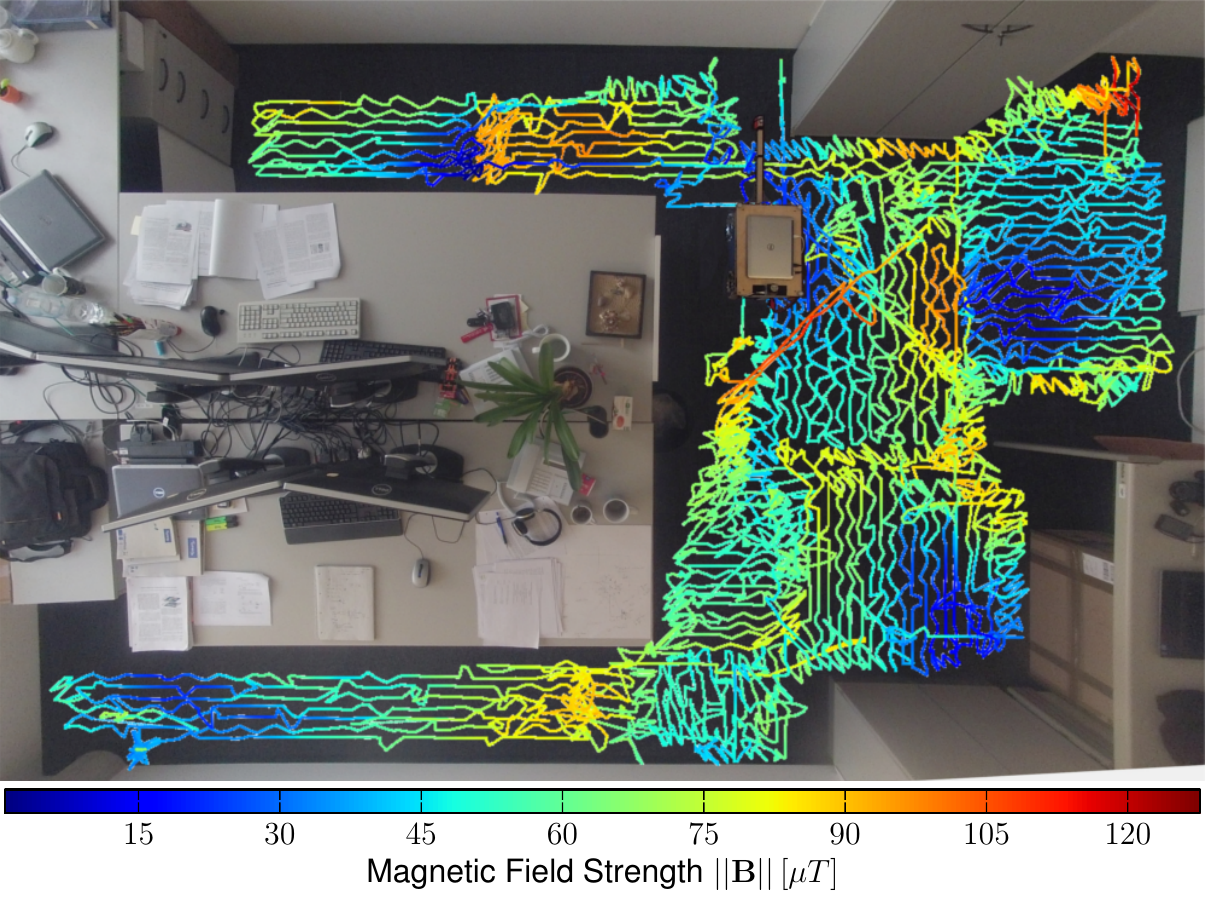
\includegraphics[width=0.45\textwidth]{images/wieser_result.png}
	\caption{
            Final result of Wieser et al. \cite{wieser_slam_indoor_2014}. It shows
            the complete coverage trajectory with measurements of the magnetic 
            field. The robot went through the office and the
            measurements have a spatial resolution of 0.05m \cite{wieser_slam_indoor_2014}.
        }
	\label{fig:wieser_result}
\end{figure}

Their program consists of four different threads. One thread processes the images by the camera
for localization and mapping and writes its result into a workspace. A thread called configuration
space mapper, processes data from the workspace and gathering data from the magnetic field sensor.
The result of that process is written into a configuration space. A path planning thread uses this
information to plan an optimal way. The last thread is called robot controller and has to perform 
the path given by the path planner while controlling the actuators of the robot. An illustration of 
that system can be seen in figure \ref{fig:wieser_system}.

\begin{figure}[h!]
	\centering
	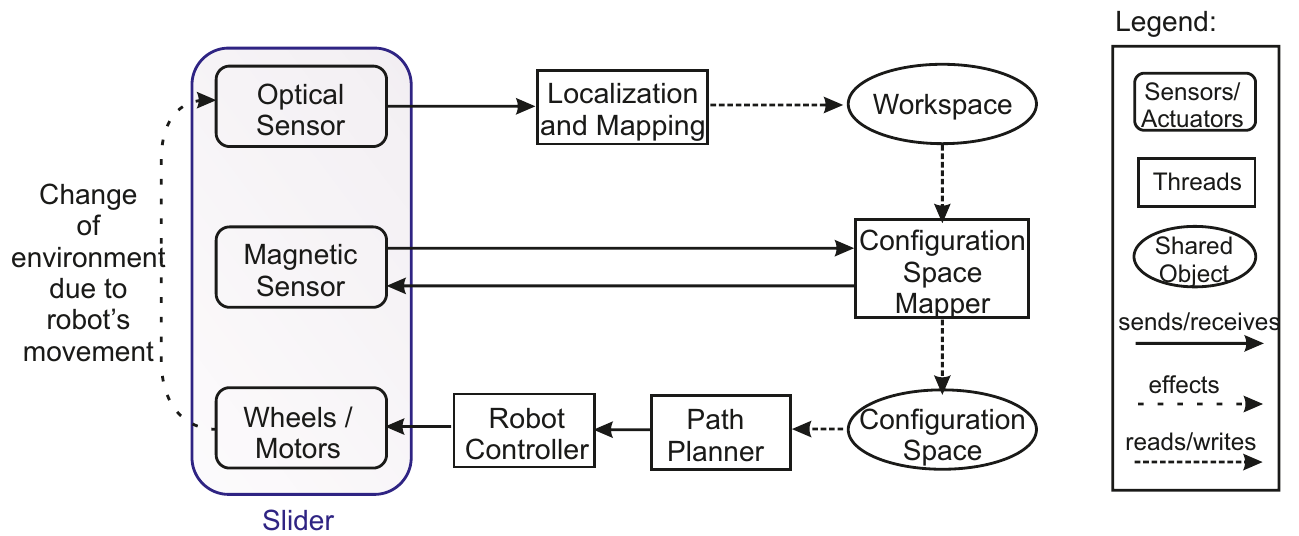
\includegraphics[width=0.5\textwidth]{images/wieser_system.png}
	\caption{
            System diagram shows the basic functionality of the approach by wieser et al. 
            \cite{wieser_slam_indoor_2014}.
        }
	\label{fig:wieser_system}
\end{figure}

\subsection{Scalable Magnetic Field SLAM}
Manon Kok and Arno Solin present in their paper an approach for scalable on-line SLAM in 3D using
magnetic field and gaussian processes \cite{kok_scalable_2018}. An example is shown
in figure \ref{fig:kok_3d}. In their work they had to face some problems which are already mentioned 
before. Approximate the underlying function of the magnetic field with gaussian processes. Handle 
large scale data because of on-line requirements. Using physical phenomena instead of images for 
SLAM approaches.

\begin{figure}[h!]
	\centering
	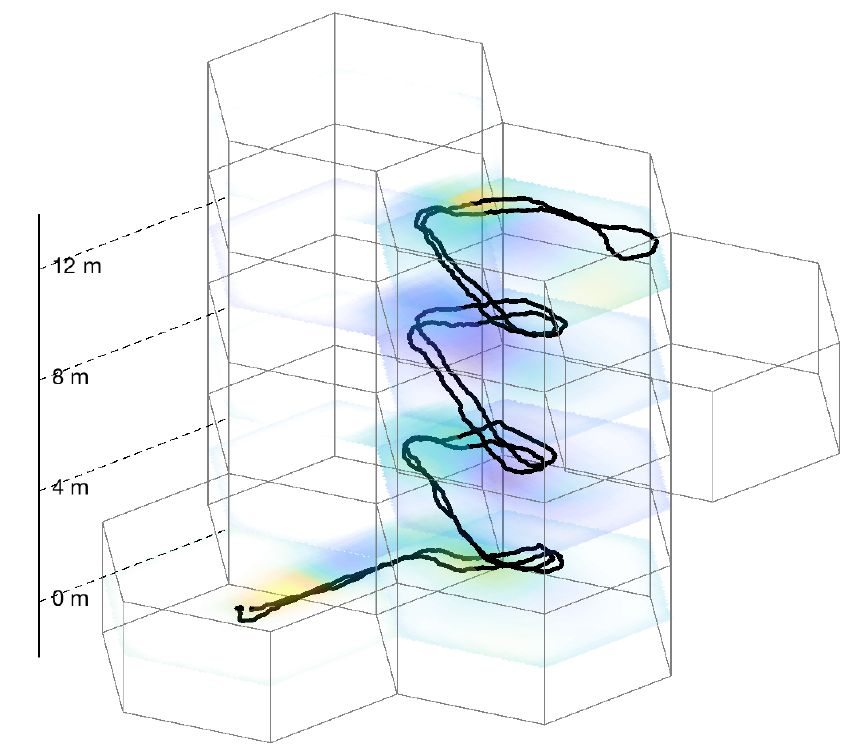
\includegraphics[width=0.45\textwidth]{images/kok_3d.png}
	\caption{
        Example by Manon Kon and Arno Solin showing 3D SLAM using magnetic field.
        The dataset was recorded at the University of Cambridge at the stairs of
        the Engineering Department \cite{kok_scalable_2018}.
        }
	\label{fig:kok_3d}
\end{figure}

To approximate the magnetic field, they use a combination of two kernels, the linear and squared
exponential kernel and a mean centered around zero \cite{kok_scalable_2018}. That leads to the 
following gaussian process.
$$
GP(0, k_{lin}(x_i, x_j) + k_{se}(x_i, x_j)) \text{ with}
$$
$$
k_{lin}(x_i, x_j) = \sigma_{lin}^2 x_i^T x_j, 
$$
$$
k_{se} = \sigma_{se}^2 \exp 
\begin{pmatrix}
    -\frac{||x_i - x_j||^2}{2l^2}
\end{pmatrix}
$$

To face the problem of on-line requirements, they divided the 3D space into hexagonal blocks
(See Figure \ref{fig:kok_3d} and \ref{fig:kok_example}). For each block there is a gaussian 
process for all data points within this block. This makes the covariance matrix for a block
much smaller than one large one. Every time a measurement is taken at a position where no hexagonal 
block exists, a new block will be created. Through that approach it is possible to do SLAM on the 
magnetic field in real time. A demonstration for that is given by them in a video they produced 
\cite{kok_scalable_2018}.

\begin{figure}[h!]
	\centering
	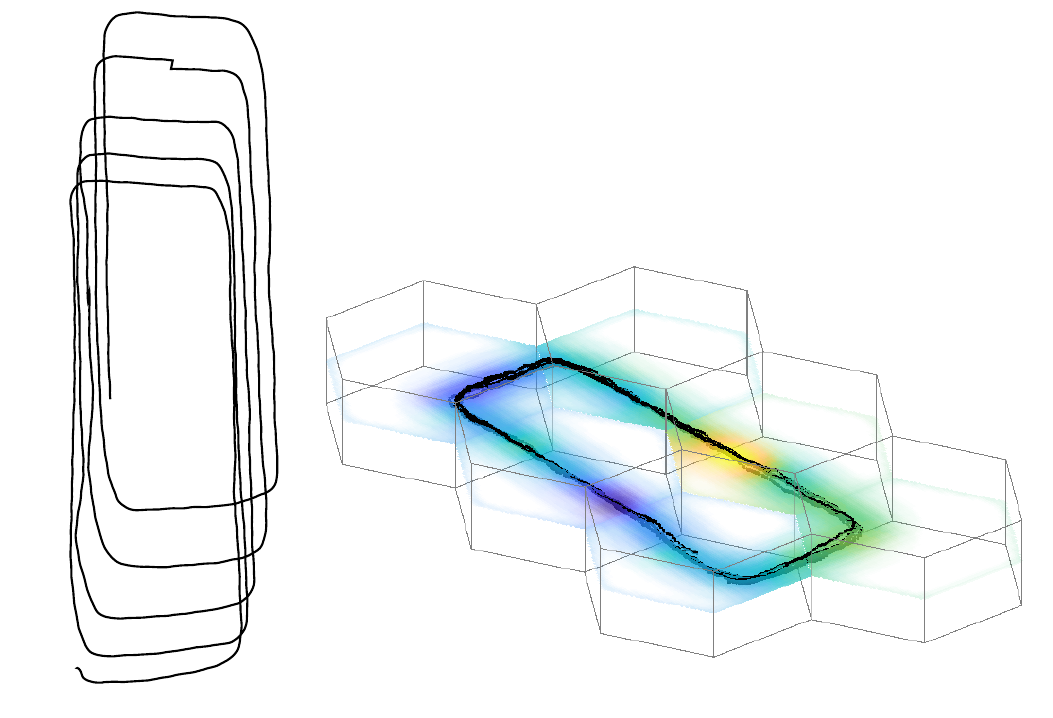
\includegraphics[width=0.5\textwidth]{images/kok_example.png}
	\caption{
        Performance demonstration of the SLAM algorithm by Kok and Solin \cite{kok_scalable_2018}.
        The trajectory on the left shows the odometrie data collected by a iPhone 6s and next to it
        the resulting trajectory with the approximated magnetic field.
        }
	\label{fig:kok_example}
\end{figure}

As mentioned in chapter \ref{chap:slam} current state of the art approaches of SLAM using graph-based
techniques. Kok and Solin don't use a graph-based approach. They choose a combination of Kalman
and particle filtering. The Kalman filter is used for update measurements and the particle filter
for predictions in time. For more information, a description of the algorithm can be found in their
paper \cite{kok_scalable_2018}. A performance demonstration is shown in figure \ref{fig:kok_example}.

\subsection{Terrain Field SLAM}
\label{chap:terrain_field}
One interesting approach from Hyeonwoo Yu and Beomhee Lee deals with terrain field SLAM \cite{yu_terrain_2018}. 
They used the vibrations obtained from the robot, which are caused by the interaction between the terrain and 
the mobile robot, as the physical phenomenon for SLAM. Their experimental setup containing the robot and an
area with different subsurfaces which can be seen in figure \ref{fig:yu_setup}.

\begin{figure}[h!]
	\centering
	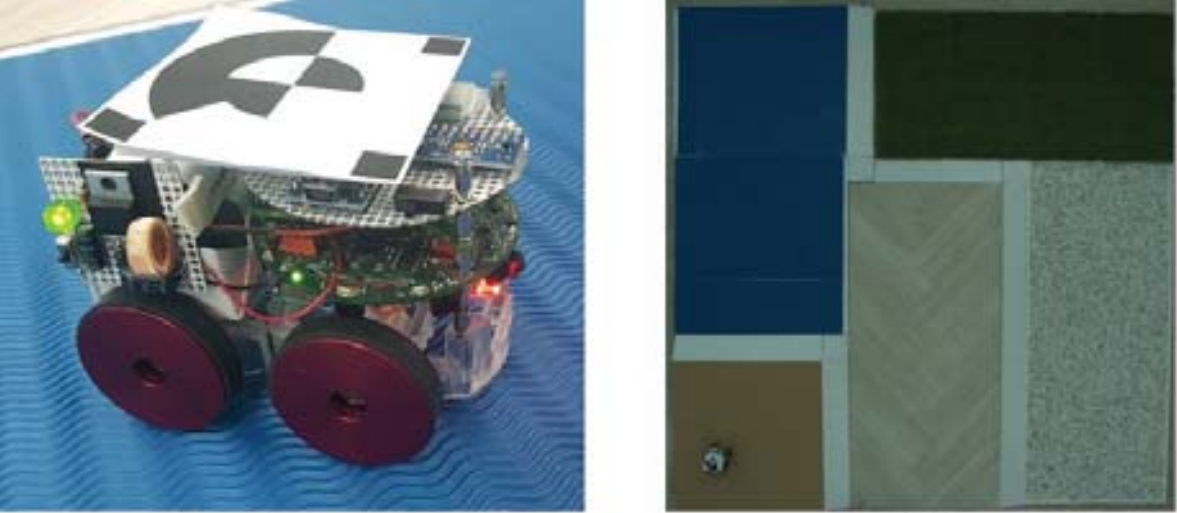
\includegraphics[width=0.5\textwidth]{images/yu_setup.png}
	\caption{
        Illustration of the setup by Yu and Lee. The mobile robot at the left and
        on the right the environment for the robot to move in. The environment containing
        five different subsurfaces \cite{yu_terrain_2018}.
        }
	\label{fig:yu_setup}
\end{figure}

Also, Yu and Lee used gaussian processes to infer the terrain field. Although, they don't face the
problem of doing SLAM and gaussian process regression on-line. A performance example of their approach
is shown in figure \ref{fig:yu_performance}. There is a little derivation over time, but
for the given terrain field the result is considerable \cite{yu_terrain_2018}.

\begin{figure}[h!]
	\centering
	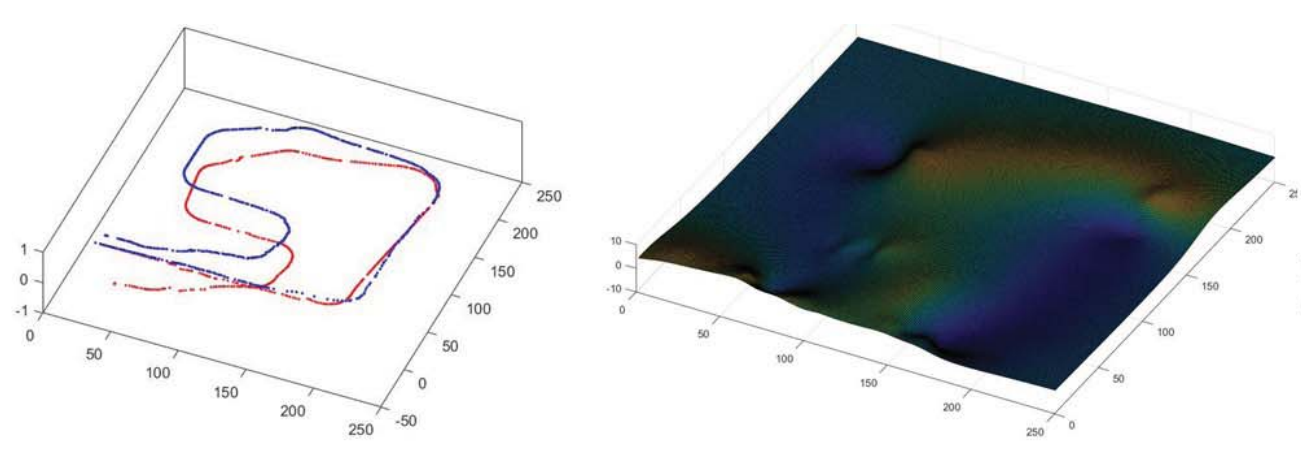
\includegraphics[width=0.5\textwidth]{images/yu_performance.png}
	\caption{
        Performance illustration of the terrain based SLAM approach by Yu and Lee \cite{yu_terrain_2018}.
        Robot trajectory in red on the left and ground truth in blue. On the right inferred terrain field.
        }
	\label{fig:yu_performance}
\end{figure}

\subsection{Uncertain Inputs with Gaussian Processes}
\label{chap:uncertain_inputs}
As mentioned in chapter \ref{chap:gaussian} uncertain inputs are not a part of standard gaussian processes
\cite{damianou_variational_2014}. So researchers have to face that problem. One team which did that is 
Andreas C. Damianou et al. First they modeled the uncertain input as:
$$
z_i \sim \mathcal{N}(x_i, \sigma_{noise})
$$
Which leads to a gaussian prior distribution over $X$:
$$
p(X|Z) = \prod_{i=1}^{\infty} \mathcal{N}(x_i| z_i, \sigma_{noise})
$$
That prior distribution they combining with the gaussian process latent variable model to handle
uncertain inputs. As an example they propagating frames in videos. For that they choose a 
fix windows size and use the frames as input for forecasting new frames. Although, frames
of the video don't have to be noisy the propagated frames are. This propagated frames are the input 
for the next time steps and because they were forecasted they are uncertain. With gaussian processes 
it is also possible to calculate the uncertainty and variance of the propagated frames which is useful 
for handling uncertain input. An example is shown in figure \ref{fig:damianou_example}.

\begin{figure}[h!]
	\centering
	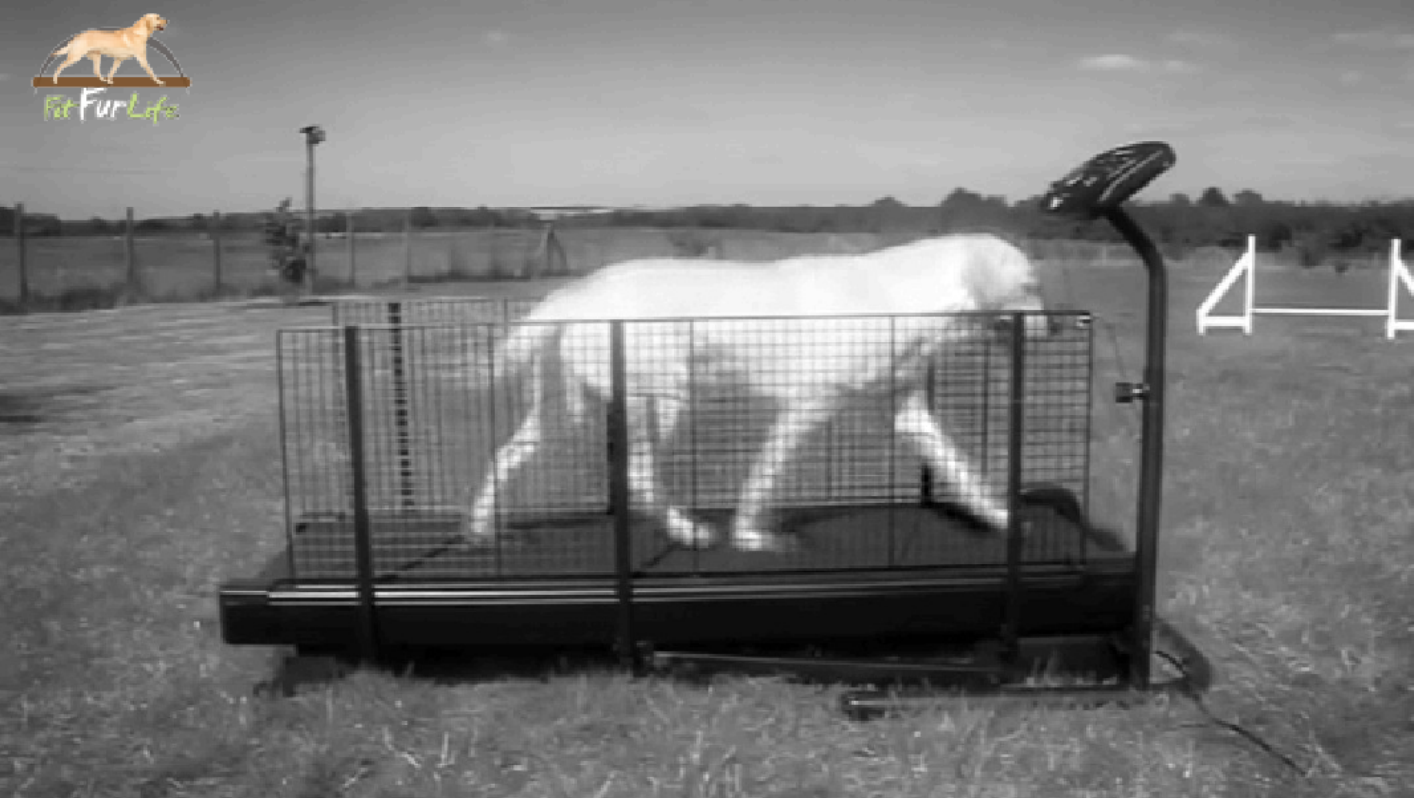
\includegraphics[width=0.425\textwidth]{images/damianou_example_1.png}
	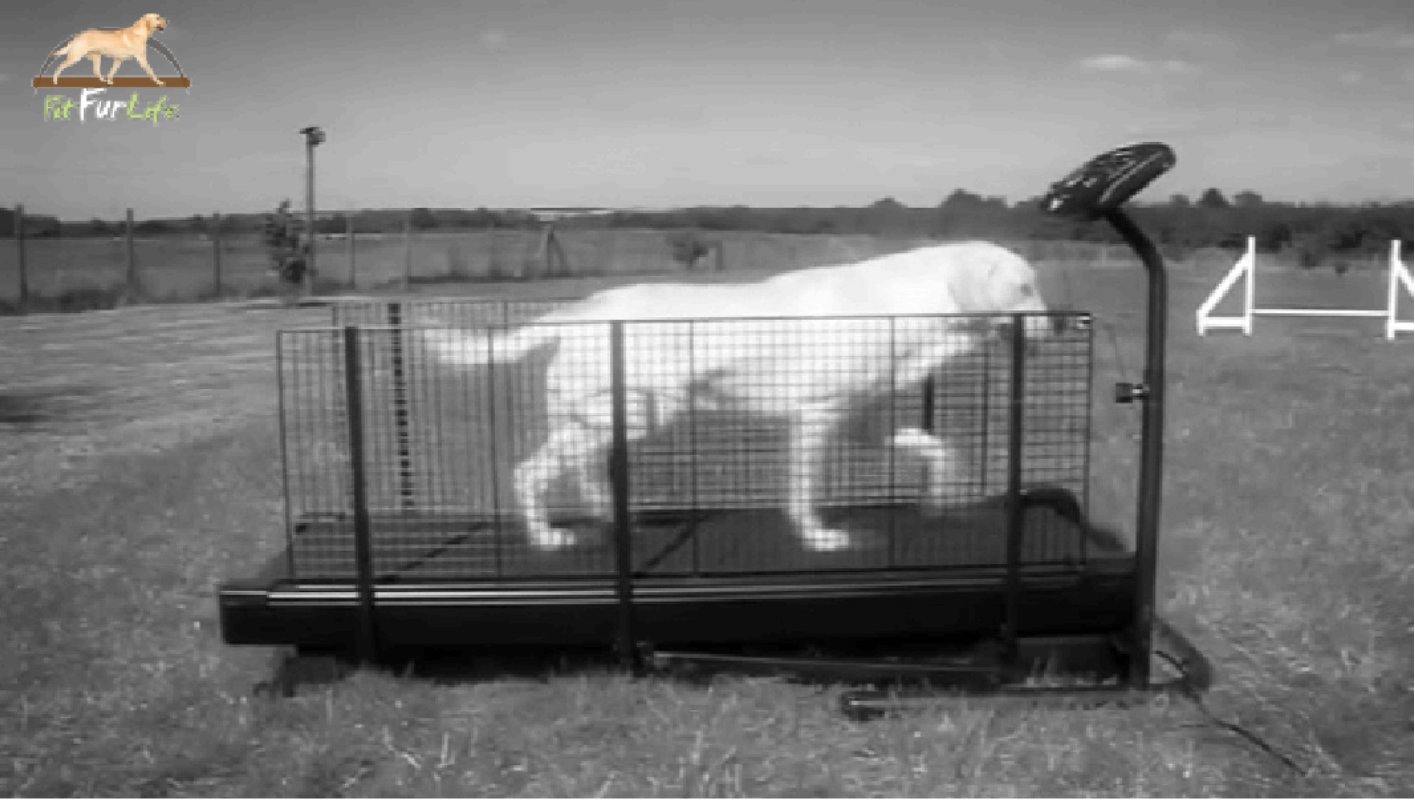
\includegraphics[width=0.425\textwidth]{images/damianou_example_2.png}
	\caption{
		Propagation demonstration of video frames. Top image shows an example
		frame of the input window for propagating the next frame (bottom). 
        }
	\label{fig:damianou_example}
\end{figure}